VLC is uitgegroeid tot een cross-platform multimedia speler die veel gebruikt wordt om films mee te kijken. VLC draait op Linux, Mac OS X en Windows. VLC kan films ook spelen vanaf CD, DVD en BluRay. Het ondersteunt vele codecs en bestandsformaten. VLC kan je ook als server gebruiken om films te streamen over het netwerk.

\begin{center}
\begin{figure}[H]
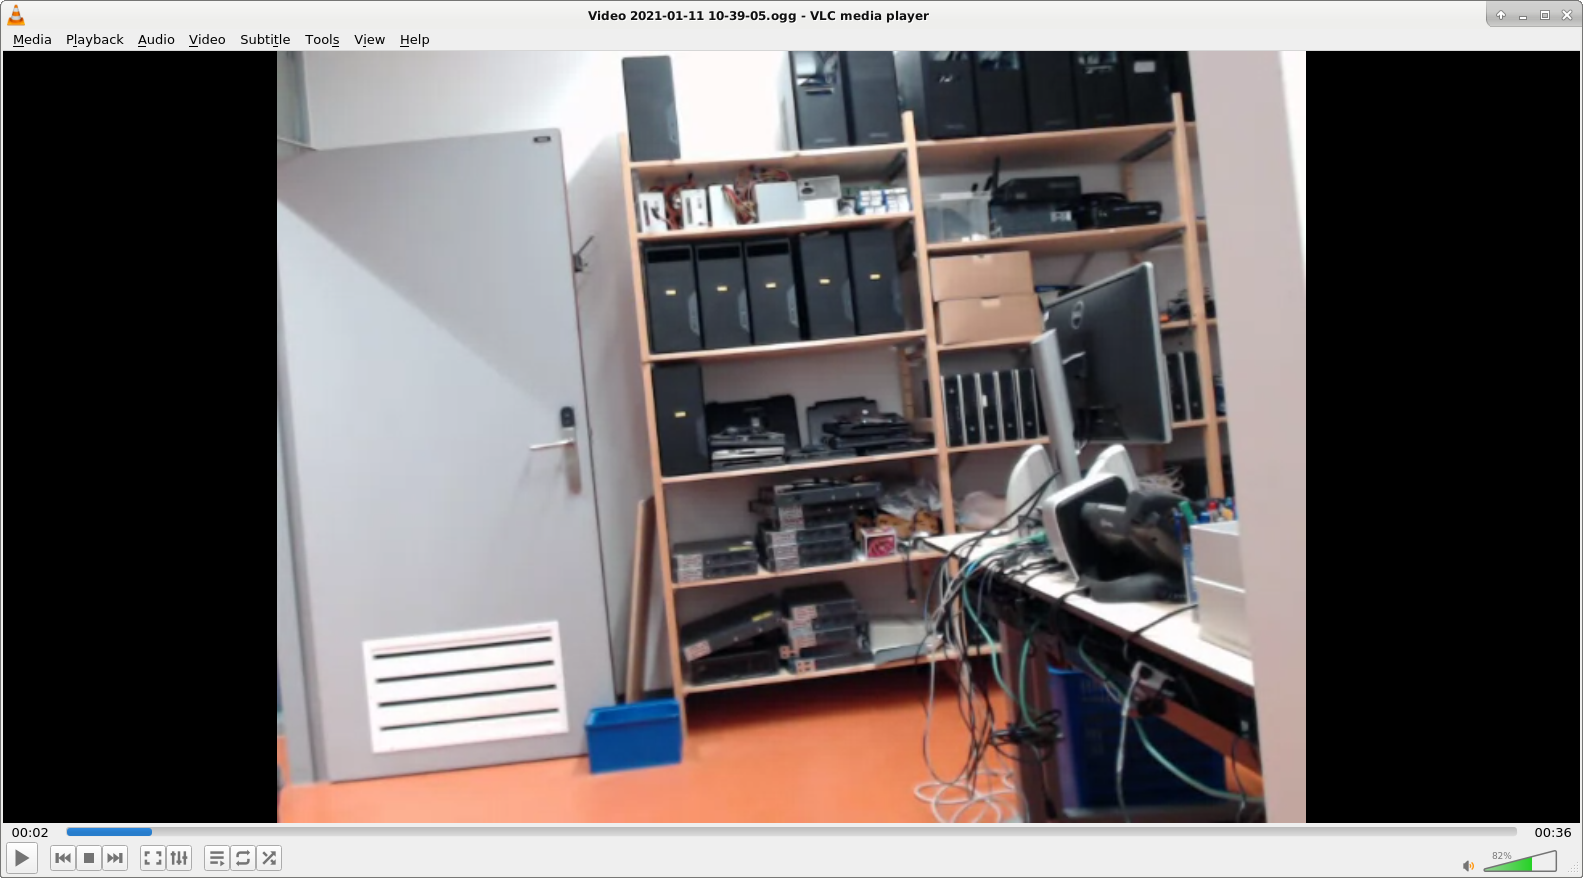
\includegraphics[width=0.9\textwidth]{VLC-working.png}
\caption{VLC}
\end{figure}
\end{center}
